\documentclass[11pt,t]{beamer}
\usetheme{Malmoe}
\usepackage[utf8]{inputenc}
\usepackage{amsmath}
\usepackage{amsfonts}
\usepackage{amssymb}
\usepackage[all,cmtip]{xy}
\usepackage{pgfpages}
\usepackage{graphicx}

\pgfpagesuselayout{resize to}[letterpaper,landscape,border shrink=5mm]
\newenvironment{amatrix}[1]{%
  \left[\begin{array}{@{}*{#1}{c}|c@{}}
}{%
  \end{array}\right]
}
\DeclareMathOperator{\rank}{rank}
\DeclareMathOperator{\minor}{minor}
\DeclareMathOperator{\cof}{cof}
\DeclareMathOperator{\adj}{adj}
\DeclareMathOperator{\spn}{span}

\newcommand{\R}{\mathbb{R}}
\newcommand{\abs}[1]{\lvert #1\rvert}
\newcommand{\len}[1]{\lVert #1\rVert}
\newcommand{\dotp}{\boldsymbol{\cdot}}
\newcommand{\comp}[2]{\operatorname{comp}_{\vec{#1}}\vec{#2}}
\newcommand{\proj}[2]{\operatorname{proj}_{\vec{#1}}\vec{#2}}
%\geometry{landscape,paper=letterpaper}
\beamertemplatenavigationsymbolsempty
\date{}
\author{Math 1410 Linear Algebra}
\title{Vectors in $\R^n$}
%\setbeamercovered{transparent} 
%\setbeamertemplate{navigation symbols}{} 
%\logo{} 
%\institute{} 
%\date{} 
%\subject{} 
\begin{document}
\begin{frame}
\titlepage
\end{frame}

%\begin{frame}
%\tableofcontents
%\end{frame}
\begin{frame}
\frametitle{A note on software}

Visualizing objects (vectors, lines, planes, etc.) in 3 dimensions can be tricky on paper. Fortunately, these days we're equipped with all kinds of computer software that helps us with these visualizations. Some software, like Mathematica or Maple, is very good but also very expensive. (You might check to see what's available in the computer labs on campus.) There are also lots of free options, including many interactive websites. You might find that simple Google searches (like ``3D vector visualization'') turn up lots of options.

I'll be using software in class called \alert{Geogebra}. If you want to try it yourself, it's free, open-source software available for Windows, OSX, and Linux. You can download it at geogebra.org.
\end{frame}
\section{Vectors: Geometric and Algebraic}
\subsection{Euclidean spaces}
\begin{frame}
\frametitle{Cartesian coordinates}
\begin{itemize}
\item Our ``base'' number system is the \alert{real numbers} $\R$.
\item Definition of $\R$ complicated - includes rational (fraction) and irrational numbers.
\item Visualize as ``number line'' -- geometrically one-dimensional.
\item Define $\R^2 = \{(x,y)\,|\, x,y\in\R\}$ -- set of \alert{ordered pairs} of real numbers.
\item \alert{Cartesian plane} visualizes $\R^2$ using two ``coordinate axes''.
\end{itemize}
\end{frame}
\begin{frame}
\frametitle{The set $\R^n$}
We can extend Descartes' construction to define the set
\[
\R^n = \{(x_1,x_2,\ldots, x_n) \,|\, x_i\in\R, i=1,\ldots, n\}.
\]
This is often referred to as ``$n$-dimensional Euclidean space''. (The adjective \alert{Euclidean} refers to the geometric structure of lines and planes.)

We can only visualize $\R^n$ for $n=1,2,$ or 3.
\end{frame}
\begin{frame}
\frametitle{Distance in $\R^n$}

The \alert{distance} between two points $x,y\in\R$ is given by
\[
d(x,y) = \abs{x-y},
\]
where $\abs{a}$ denotes the \alert{absolute value} of $a\in \R$. Notice that $\abs{x-y} = \sqrt{(x-y)^2}$.

\bigskip

In $\R^2$, distance is given by the Pythagorean Theorem:
\[
d((x_1,y_1),(x_2,y_2)) = \sqrt{(x_1-x_2)^2+(y_1-y_2)^2}.
\]

We can prove that the same pattern holds in $\R^3$:
\[
d((x_1,y_1,z_1),(x_2,y_2,z_2)) = \sqrt{(x_1-x_2)^2+(y_1-y_2)^2+(z_1-z_2)^2}.
\]
We \alert{define} distance in $\R^n$ for $n\geq 4$ by insisting that this pattern continues.

\end{frame}
\begin{frame}
\frametitle{Vectors, geometric and algebraic}
Our interest in Chapter 4 is the study of \alert{vectors}. The meaning of the term ``vector'' varies depending on the context:
\begin{itemize}
\item Geometry/physics: a quantity with both \alert{magnitude} and \alert{direction}. (Basically, an arrow.) Think of velocity, force, etc.
\item Algebra: quantities that can be added together, and multiplied by numbers (scalars), subject to certain rules.
\item Data analytics: ordered arrays of information that can be manipulated.
\item And so on...
\end{itemize}
The third point above isn't all that different from the second. We'll be interested in seeing how the second point is connected to the first.
\end{frame}
\subsection{Geometric vectors}
\begin{frame}
\frametitle{Geometric vectors}

A \alert{geometric vector} in $\R^n$ is visualized as an arrow. We if the ``tail'' of our arrow/vector $\vec{v}$ is at a point $P=(x_1,\ldots x_n)$ and the ``tip'' is at a point $Q=(y_1,\ldots, y_n)$, we write $\vec{v}=\overrightarrow{PQ}$.

Viewed geometrically, a vector is determined by its \alert{length} (\alert{magnitude}) and \alert{direction}, but not its {\em location}. Thus, if $R=(x_1+a_1,\ldots, x_n+a_n)$ and $S=(y_1+a_1,\ldots, y_n+a_n)$ for some constants $a_1,\ldots, a_n$, then $\overrightarrow{RS}=\overrightarrow{PQ}$.

\begin{example}

\end{example}
\end{frame}
\begin{frame}
\frametitle{Numerical representation of vectors}

Let $\vec{v}=\overrightarrow{PQ}$ as on the previous slide. Note that all the information about $\vec{v}$ is contained in the differences $y_1-x_1,y_2-x_2,\ldots,y_n-x_n$. We represent $\vec{v}$ numerically by
\[
\vec{v} = \langle y_1-x_1,y_2-x_2,\ldots,y_n-x_n\rangle.
\]
Notice that this representation does not depend on the location of $\vec{v}$:
\end{frame}
\begin{frame}
\frametitle{Position vectors}

Since the location of a geometric vector doesn't matter, it's often convenient to locate the tail of the vector at the origin $O=(0,0,\ldots, 0)$. If $P=(x_1,x_2,\ldots, x_n)$ is any other point in $\R^n$, we have the corresponding \alert{position vector}
\[
\vec{p} = \overrightarrow{OP} = \langle x_1,x_2,\ldots, x_n\rangle.
\]

Note: there is a ``one-to-one'' correspondence between points in $\R^n$ and vectors in $\R^n$. For every point $P$ we have the corresponding position vector $\vec{p}$, and vice versa.
\end{frame}
\begin{frame}
\frametitle{Length of a vector}

The \alert{length}, or \alert{magnitude} of a vector $\vec{v}$ is denoted by $\len{\vec{v}}$. If $\vec{v}=\overrightarrow{PQ}$, then $\len{\vec{v}}$ is simply the distance from $P$ (the tail of $\vec{v}$) to $Q$ (the tip). Thus,
\[
\len{\vec{v}} = \sqrt{v_1^2+\cdots +v_n^2}=\sqrt{(x_1-y_1)^2+\cdots+(x_n-y_n)^2},
\]
where the numbers $v_i = x_i-y_i$, $i=1,2,\ldots, n$, are called the \alert{components} of $\vec{v}$.
\end{frame}
\begin{frame}
\frametitle{Addition of geometric vectors}

Geometric vectors are added according to the ``tip-to-tail'' or ``parallelogram'' rule. We can sketch the procedure as follows:

\end{frame}
\begin{frame}
\frametitle{Scalar multiplication of geometric vectors}

Let $c\in\R$ be a real number, and let $\vec{v}$ be a vector in $\R^n$. The scalar multiple $c\vec{v}$ is defined as follows:

\begin{itemize}
\item If $c>0$, then $c\vec{v}$ points in the \alert{same} direction as $\vec{v}$, and has length $\len{c\vec{v}} = c\len{\vec{v}}$.
\item If $c=0$, then $c\vec{v}$ is the ``zero vector'' $\vec{0}$.
\item If $c<0$, then $c\vec{v}$ points in the \alert{opposite} direction as $\vec{v}$, and has length $\len{c\vec{v}} = (-c)\len{\vec{v}}$.
\end{itemize}

Notes:
\begin{enumerate}
\item We can sum up all of the above with the rule $\len{c\vec{v}} = \abs{c}\len{\vec{v}}$.
\item The zero vector is a little weird. It has magnitude zero, but \alert{no direction}.
\end{enumerate}
\end{frame}
\subsection{Algebraic vectors}
\begin{frame}
\frametitle{Algebraic vectors}
We've already met algebraic vectors. Let's let $\R^{n,1}$ denote the set of all $n\times 1$ column vectors
\[
\vec{x} = \begin{bmatrix}
x_1\\x_2\\\vdots \\x_n
\end{bmatrix}=\begin{bmatrix}
x_1&x_2&\cdots &x_n\end{bmatrix}^T
\]
We define
\[
\vec{x}+\vec{y} = \begin{bmatrix}
x_1\\x_2\\\vdots \\x_n
\end{bmatrix}+\begin{bmatrix}
y_1\\y_2\\\vdots \\y_n
\end{bmatrix} = \begin{bmatrix}
x_1+y_1\\x_2+y_2\\\vdots \\x_n+y_n
\end{bmatrix} \text{ and } c\vec{x}=c\begin{bmatrix}
x_1\\x_2\\\vdots \\x_n
\end{bmatrix}=\begin{bmatrix}
cx_1\\cx_2\\\vdots \\cx_n
\end{bmatrix},
\]
where $c$ is a scalar. (This was our definition for matrices in general.)
\end{frame}
\begin{frame}
\frametitle{Examples}
\end{frame}
\begin{frame}
\frametitle{Properties of vector algebra}
The addition and scalar multiplication of vectors follows the following rules:

For any vectors $\vec{x},\vec{y},\vec{z}$ and scalars $c,d\in\R$,
\begin{enumerate}
\item $\vec{x}+\vec{y} = \vec{y}+\vec{x}$
\item $\vec{x}+(\vec{y}+\vec{z}) = (\vec{x}+\vec{y})+\vec{z}$
\item $\vec{x}+\vec{0} = \vec{x}$, where $\vec{0} = \begin{bmatrix}0&0&\cdots&0\end{bmatrix}^T$
\item $\vec{x}+(-\vec{x})=\vec{0}$, where $-\vec{x} = \begin{bmatrix}-x_1&-x_2&\cdots&-x_n\end{bmatrix}^T$
\item $1\cdot\vec{x}=\vec{x}$
\item $c(d\vec{x}) = (cd)\vec{x}$
\item $c(\vec{x}+\vec{y}) = c\vec{x}+c\vec{y}$
\item $(c+d)\vec{x} = c\vec{x}+d\vec{x}$.
\end{enumerate}
\end{frame}
\begin{frame}
\frametitle{Vector spaces}
Whenever we have a set of objects on which we can define an addition and scalar multiplication satisfying the same 8 rules as vectors in $\R^n$, we call that set a \alert{vector space}.

There are lots of examples: $\R^n$, of course, but also the space of all $m\times n$ matrices, and the space of all polynomials of degree less than or equal to $k$ for some $k$. (These are ``finite-dimensional'' vectors spaces.)

Other examples include the space of all real-valued functions defined on some interval $[a,b]$, and the space of all sequences $(a_1,a_2,a_3,\ldots)$. (These are {\em infinite-dimensional} vector spaces.)

\bigskip

For Math 1410, the only vector spaces are $\R^n$, for $n=1,2,3\ldots$. For general vector spaces, take Math 3410.
\end{frame}
\begin{frame}\frametitle{Algebraic vs. Geometric}
 We've defined vectors in $\R^n$ in two ways:
\begin{itemize}
 \item Geometric vectors $\vec{v}=\overrightarrow{PQ} = \langle y_1-x_1,\ldots, y_n-x_n\rangle$, where $P=(x_1,\ldots, x_n)$ is the point at the tip of the vector, and $Q=(y_1,\ldots, y_n)$ is the point at the tail.
 \item Algebraic vectors $\vec{v} = \begin{bmatrix}v_1\\\vdots\\v_n\end{bmatrix}$, where $v_1,\ldots, v_n\in \R$ are real numbers.
\end{itemize}
Goal: adding geometric vectors is the same as adding algebraic vectors, and the same is true for scalar multiplication.
\end{frame}
\begin{frame}\frametitle{Examples}
 
\end{frame}
\begin{frame}\frametitle{Linear combinations}
 One of the most fundamental concepts in Linear Algebra is the \alert{linear combination}.

 Let $\vec{v}_1,\vec{v}_2,\ldots,\vec{v}_k$ be vectors in $\R^n$ and let $c_1, c_2, \ldots, c_k$ be scalars. A vector $\vec{v}$ is a linear combination of the vectors $\vec{v}_i$ if
\[
 \vec{v} = c_1\vec{v}_1+c_2\vec{v}_2+\cdots + c_k\vec{v}_k
\]

\end{frame}
\begin{frame}\frametitle{Algebraic examples}
 
\end{frame}
\begin{frame}\frametitle{Geometric examples}
 
\end{frame}
\begin{frame}\frametitle{Another example}
 \alert{Problem:} given $\vec{u} = \begin{bmatrix}2\\-3\\4\end{bmatrix}$ and $\vec{v} = \begin{bmatrix}-1\\2\\3\end{bmatrix}$, find the following points:
\begin{enumerate}
 \item $P$, half-way between the tip of $\vec{u}$ and the tip of $\vec{u+v}$.
 \item $Q$, half-way between the tip of $\vec{v}$ and the tip of $\vec{u+v}$.
\end{enumerate}

\end{frame}

\begin{frame}
\frametitle{Summary of results so far}

\alert{Recall}: Last week we studied the algebraic and geometric properties of vectors in $\mathbb{R}^n$. We had three basic objects:
\begin{enumerate}
\item \alert{Points} in $\R^n$: $P = (x_1,x_2,\ldots, x_n)$
\item \alert{Geometric vectors} in $\R^n$: $\vec{v} = \langle x_1,x_2,\ldots, x_n\rangle$
\item \alert{Algebraic vectors} in $\R^n$: $\vec{v} = \begin{bmatrix}
x_1\\x_2\\\vdots\\x_n
\end{bmatrix}$
\end{enumerate}
Note that all three concepts provide the \alert{same information}:
\begin{itemize}
\item We can identify points $P$ with position vectors $\vec{p}$
\item Component-wise (algebraic) addition of vectors corresponds to ``tip-to-tail'' (geometric) addition.
\item Component-wise (algebraic) scalar multiplication also agrees with geometric scalar multiplication.
\end{itemize}
\end{frame}
\begin{frame}\frametitle{Linear independence}
 We say that a set of vectors $\vec{v}_1,\vec{v}_2,\ldots, \vec{v}_k$ is \alert{linearly dependent} if one of the vectors can be written as a linear combination of the other vectors; for example, if
\[
 \vec{v}_1 = c_2\vec{v}_2+\cdots+c_k\vec{v}_k
\]
for scalars $c_2,\ldots, c_k$.

 This tells us we don't really need the first vector, since we can get it from the other ones.

 On the other hand, our vectors are \alert{linearly independent} if the above is impossible. Equivalently, the only way we can have
\[
 c_1\vec{v}_1+c_2\vec{v}_2+\cdots + c_k\vec{v}_k=\vec{0}
\]
is if $c_1=0, c_2=0,\ldots, c_k=0$.
\end{frame}
\begin{frame}\frametitle{Example}
 
\end{frame}
\begin{frame}\frametitle{Example}
 
\end{frame}

\begin{frame}\frametitle{Span}
 The \alert{span} of vectors $\vec{v}_1,\ldots, \vec{v}_k$ in $\R^n$ is the set of all possible linear combinations we can form from these vectors. Thus,
\[
 \vec{w}\in\spn\{\vec{v}_1,\ldots, \vec{v}_k\}
\]
if and only if
\[
 \vec{w} = c_1\vec{v}_1+\cdots + c_k\vec{v}_k
\]
for scalars $c_1,\ldots, c_k$.
\end{frame}
\begin{frame}\frametitle{Example}
Let $\vec{u} = \begin{bmatrix}2&-1&4\end{bmatrix}$ and $\vec{v} = \begin{bmatrix}-1&3&1\end{bmatrix}$. Describe:
\begin{enumerate}
 \item $\spn\{\vec{u}\}$
 \item $\spn\{\vec{u},\vec{v}\}$
\end{enumerate}
 
\end{frame}
\begin{frame}\frametitle{Subspaces}
 A \alert{subspace} of $\R^n$ is a subset $U\subseteq \R^n$ that satisfies all of the 8 vector space properties described earlier. One can show that $U$ is a subspace if:
\begin{enumerate}
 \item $\vec{0}$ belongs to $U$.
 \item If $\vec{u}_1,\ldots, \vec{u}_k$ are vectors in $U$, then any linear combination $c_1\vec{u}_1+\cdots + c_k\vec{u}_k$ also belongs to $U$.
\end{enumerate}
 Consequence: every subspace can be written as the span of some vectors.
\end{frame}

\section{Lines and dot products}
\subsection{Lines in $\R^3$}
\begin{frame}\frametitle{Lines in $\R^2$}
 We know many ways to describe a line in the plane: two points, point and slope, $y=mx+b$, $y-y_0 = m(x-x_0)$, etc.
\end{frame}
\begin{frame}\frametitle{Lines in $\R^3$ - I}
 In three dimensions, two points still determine a line, but ``slope'' has no meaning.

 However, given points $P$ and $Q$, we have a \alert{direction}: the vector $\overrightarrow{PQ}$. This leads to a \alert{vector equation} of a line:
\end{frame}
\begin{frame}\frametitle{Example}
 Find the line in $\R^3$ through the points $P=(0,1,3)$ and $Q=(2,-1,4)$.
\end{frame}

\begin{frame}\frametitle{Lines in $\R^3$ - II}
 Note we have various ways of describing a line again: two points, point and \alert{direction}, or a vector equation. We often are also interested in \alert{parametric equations} of a line.
\end{frame}
\begin{frame}
\frametitle{Lines as subspaces}

\alert{Remark:} If $\vec{v}$ is a nonzero vector in $\R^n$, then
\[
U=\spn\{\vec{v}\} = \{t\vec{v} \,|\, t\in\R\}
\]
 is a line through the origin. It is also a \alert{subspace}. In fact, all ``one-dimensional'' subspaces of $\R^n$ are of this form.
\end{frame}
\subsection{Dot products}
\begin{frame}
\frametitle{Dot products}

The \alert{dot product} (or scalar product) of two vectors $\vec{u} = \begin{bmatrix}
u_1&u_2&\cdots &u_n
\end{bmatrix}^T$, $\vec{v} = \begin{bmatrix}
v_1&v_2&\cdots &v_n
\end{bmatrix}^T$ is defined \alert{algebraically} by
\[
\vec{u}\dotp \vec{v} = u_1v_1+u_2v_2+\cdots + u_nv_n = \sum_{i=1}^n u_iv_i.
\]
If we view $\vec{u}$ and $\vec{v}$ as \alert{geometric} vectors, then we define
\[
\vec{u}\dotp \vec{v} = \len{\vec{u}}\len{\vec{v}}\cos\theta,
\]
where $\theta$ is the angle between the two vectors.
\end{frame}
\begin{frame}
\frametitle{Examples}

\end{frame}
\begin{frame}
\frametitle{Algebraic definition = geometric definition}
\begin{theorem}
For any vectors $\vec{u} , \vec{v}$ in $\R^n$, the geometric and algebraic definitions  of the dot product coincide. That is,
\[
\vec{u}\dotp\vec{v} = u_1v_1+\cdots + u_nv_n = \len{\vec{u}}\len{\vec{v}}\cos\theta.
\]
The proof uses the \alert{law of cosines}: for any triangle with sides of length $a,b,c$, if $\theta$ is the interior angle opposite the side of length $c$, then
\[
c^2 = a^2+b^2-ab\cos\theta.
\]
\end{theorem}
\end{frame}
\begin{frame}
\frametitle{Properties of the dot product}
\begin{theorem}
For any vectors $\vec{u},\vec{v},\vec{w}$ and any scalars $a,b\in\R$, we have:
\begin{enumerate}
\item $\vec{u}\dotp\vec{v} = \vec{v}\dotp\vec{w}$
\item $\vec{u}\dotp(a\vec{v}+b\vec{w}) = a\vec{u}\dotp\vec{v}+b\vec{u}\dotp\vec{w}$.
\item If $\vec{u}\dotp\vec{v} = 0$ for \alert{all} vectors $\vec{v}$, then $\vec{u}=0$.
\item $\vec{u}\dotp\vec{u} = \len{\vec{u}}^2$
\item $\vec{u}\dotp\vec{u}\geq 0$, and $\vec{u}\dotp\vec{u}=0$ if and only if $\vec{u}=\vec{0}$
\item $\abs{\vec{u}\dotp\vec{v}}\leq \len{\vec{u}}\len{\vec{v}}$ (Cauchy-Schwarz inequality)
\end{enumerate}
\end{theorem}
\end{frame}
\begin{frame}
\frametitle{Some proofs}

\end{frame}
\begin{frame}
\frametitle{Examples}

\end{frame}
\begin{frame}
\frametitle{Triangle inequality}

A consequence of the Cauchy-Schwarz inequality is the \alert{triangle inequality}:
\begin{theorem}
For any vectors $\vec{u}$ and $\vec{v}$ in $\R^n$, we have
\[
\len{\vec{u}+\vec{v}}\leq \len{\vec{u}}+\len{\vec{v}}.
\]
\end{theorem}
Another result that is often useful is the ``reverse triangle inequality'':
\[
\abs{\len{\vec{u}}-\len{\vec{v}}} \leq \len{\vec{u}-\vec{v}}.
\]
\end{frame}
\begin{frame}
\frametitle{Dot product and geometry}
We saw above that $\vec{u}\dotp\vec{v} = \len{\vec{u}}\len{\vec{v}}\cos\theta$ for any vectors $\vec{u}$ and $\vec{v}$.

If we know the components of two non-zero vectors $\vec{u}$ and $\vec{v}$, then we can find the angle between them:
\[
\cos\theta = \frac{\vec{u}\dotp\vec{v}}{\len{\vec{u}}\len{\vec{v}}}.
\]
In particular, note that $\vec{u}\dotp\vec{v} = 0$ if and only if $\cos\theta = 0$; i.e.,  $\theta = \dfrac{\pi}{2}$.
\begin{definition}
We say that two vectors $\vec{u},\vec{v}$ in $\R^n$ are \alert{orthogonal} if $\vec{u}\dotp\vec{v} = 0$.
\end{definition}
\end{frame}
\begin{frame}
\frametitle{Example}
Find the angle between the vectors $\vec{u} = \begin{bmatrix}
2\\-3\\1\end{bmatrix}$ and $\vec{v} = \begin{bmatrix}
-1\\4\\-2
\end{bmatrix}$.


\end{frame}
\begin{frame}
\frametitle{Example}

Two lines $L_1$ and $L_2$ intersect at the point $P=(1,0,-2)$. If $L_1$ also passes through the point $Q=(3,5,1)$ and $L_2$ passes through the point $R=(-2,1,3)$, find the angle between the two lines.
\end{frame}
\subsection{Projections}
\begin{frame}
\frametitle{Unit vectors}

A \alert{unit vector} is a vector of length 1. Note that if $\vec{v}\neq\vec{0}$, one possible unit vector is
\[
\hat{v} = \frac{1}{\len{\vec{v}}}\vec{v}.
\]

The \alert{standard unit vectors} in $\R^n$ are the vectors $\begin{bmatrix}
1\\0\\\vdots \\0
\end{bmatrix},\begin{bmatrix}
0\\1\\\vdots\\0
\end{bmatrix},\cdots,\begin{bmatrix}
0\\0\\\vdots\\1
\end{bmatrix}.$ In $\R^3$, common notation is
\[
\hat{\imath} = \begin{bmatrix}1\\0\\0\end{bmatrix}, \hat{\jmath} = \begin{bmatrix}0\\1\\0\end{bmatrix}, \hat{k} = \begin{bmatrix}0\\0\\1\end{bmatrix}.
\]
\end{frame}
\begin{frame}
\frametitle{Components}
The dot product lets us tell ``how much'' of a vector $\vec{v}$ lies in the same direction as a vector $\vec{u}$ (i.e. how closely the two vectors are aligned).
\begin{definition}
Let $\vec{u}$ be a nonzero vector. The \alert{component} of $\vec{v}$ in the direction of $\vec{u}$ is defined by
\[
\comp{u}{v} = \frac{\vec{v}\dotp\vec{u}}{\len{\vec{u}}} = \len{\vec{v}}\cos\theta.
\]
\end{definition}
Note: we divide by $\len{\vec{u}}$ since we only care about the direction of $\vec{u}$, not its length.

\alert{Remark:} Note that components of a vector $\vec{v}$ in the direction of the standard unit vectors are just the usual components of $\vec{v}$.
\end{frame}
\begin{frame}
\frametitle{Projections}

Given vectors $\vec{u},\vec{v}$, note that $\comp{u}{v}$ is a \alert{number}. The corresponding \alert{vector} quantity is called the projection of $\vec{v}$ onto $\vec{u}$:
\begin{definition}
Let $\vec{u}$ be a nonzero vector. The \alert{projection} of $\vec{v}$ onto $\vec{u}$ is the vector $\proj{u}{v}$ defined by
\[
\proj{u}{v} = \left(\frac{\vec{u}\dotp\vec{v}}{\len{\vec{u}}^2}\right)\vec{u} = (\comp{u}{v})\hat{u},
\]
where $\hat{u} = \frac{1}{\len{\vec{u}}}\vec{u}$ is the unit vector in the direction of $\vec{u}$.
\end{definition}
Note that $\proj{u}{v}$ is the vector in the direction of $\vec{u}$ whose length is $\comp{u}{v}$.
\end{frame}
\begin{frame}
\frametitle{Orthogonal decomposition}
\begin{theorem}
Let $\vec{u}$ be a nonzero vector  in $\R^n$. Then given any vector $\vec{v}$ in $\R^n$, there exist vectors $\vec{v}_{\parallel}$ and $\vec{v}_{\perp}$ such that:
\begin{enumerate}
\item $\vec{v}_{\parallel}$ is parallel to $\vec{u}$,
\item $\vec{v}_{\perp}$ is orthogonal to $\vec{u}$, and
\item $\vec{v} = \vec{v}_\parallel+\vec{v}_\perp$.
\end{enumerate}
\end{theorem}
\end{frame}
\begin{frame}
\frametitle{Examples}
Let $\vec{u} = \begin{bmatrix}1&-2&2\end{bmatrix}^T$ and $\vec{v} = \begin{bmatrix}3&4&-1\end{bmatrix}^T$. Find:
\begin{enumerate}
\item $\comp{u}{v}$
\item $\proj{u}{v}$
\item $\vec{v}_\parallel$ and $\vec{v}_\perp$.
\end{enumerate}
\end{frame}
\begin{frame}
\frametitle{Example}

Let $L$ be the line given by $\begin{bmatrix}
x\\y\\z
\end{bmatrix} = \begin{bmatrix}
2\\1\\-3
\end{bmatrix}+t\begin{bmatrix}
4\\0\\-3
\end{bmatrix}.$ Find the point on $L$ that is closest to the point $P=(5,-3,7)$.
\end{frame}
\section{Planes and the cross product}
\subsection{Planes in $\R^3$}
\begin{frame}\frametitle{Planes in $\R^3$}
 A \alert{plane} in $\R^3$ is a flat, two-dimensional surface sitting inside of $\R^3$. (Think of a copy of $\R^2$ inside $\R^3$.) The most basic examples are the \alert{coordinate planes}:
\begin{itemize}
 \item The $xy$-plane: $\{(x,y,0)\,|\,x,y\in\R\}$, or $z=0$.
 \item The $yz$-plane: $\{(0,y,z)\,|\,y,z\in\R\}$, or $x=0$.
 \item The $xz$-plane: $\{(x,0,z)\,|\,x,z\in\R\}$, or $y=0$.
\end{itemize}
More general planes can be defined in many ways:
\begin{itemize}
 \item As a single linear equation: $ax+by+cz=d$.
 \item By specifying three points (not all on the same line).
 \item By giving two intersecting lines.
 \item As the \alert{span} of two vectors.
 \item By giving a point and a \alert{normal vector}
\end{itemize}
\end{frame}
\begin{frame}\frametitle{Scalar equation}
 Choose a point $P_0=(x_0,y_0,z_0)\in\R^3$ and a non-zero vector $\vec{n} = \begin{bmatrix}a&b&c\end{bmatrix}^T$.

 The \alert{plane} determined by $P_0$ and $\vec{n}$ is the set of all points $P$ such that the vector $\overrightarrow{P_0P}$ is \alert{perpendicular} to $\vec{n}$.
\end{frame}
\begin{frame}\frametitle{Example}
 Determine the plane through the point $P_0=(2,-3,1)$ with normal vector $\vec{n}=\langle 5,-2,3\rangle$.
\end{frame}
\begin{frame}\frametitle{Example}
 Find the shortest distance from the point $Q=(2,1,-3)$ to the plane with equation $3x-y+4z=1$.
\end{frame}
\begin{frame}\frametitle{Example}
 Describe the intersection of the planes given by $2x-y+4z=2$ and $x+2y-z=5$.
\end{frame}

\begin{frame}\frametitle{Planes as spans}
 Recall that given vectors $\vec{u}$ and $\vec{v}$, we define
\[
 \spn\{\vec{u},\vec{v}\} = \{a\vec{u}+b\vec{v} \,|\,a,b\in\R\}.
\]
Suppose we're given a plane $a(x-x_0)+b(y-y_0)+c(z-z_0)=0$ in $\R^3$. Think of this single equation as a \alert{system} of one equation in three variables. 

How would we have handled this in Chapter 1?
\end{frame}
\begin{frame}\frametitle{Planes through $(0,0,0)$ are subspaces}
 A plane through the origin is given by $ax+by+cz=0$. This is equivalent to the vector equation
\[
 \begin{bmatrix}x\\y\\z\end{bmatrix} = s\begin{bmatrix}-b\\a\\0\end{bmatrix}+t\begin{bmatrix}-c\\0\\a\end{bmatrix}
\]

\end{frame}
\begin{frame}\frametitle{Returning to the scalar equation}
Suppose we are given a plane through $P_0=(x_0,y_0,z_0)$ such that the vectors $\vec{u}=\begin{bmatrix}u_1&u_2&u_3\end{bmatrix}^T$ and $\vec{v}=\begin{bmatrix}v_1&v_2&v_3\end{bmatrix}^T$ are parallel to the plane. How can we recover the scalar equation?
 
\end{frame}
\subsection{The cross product}
\begin{frame}\frametitle{The cross product}
 There are two ways to define the \alert{cross product} $\vec{u}\times \vec{v}$ of two vectors in $\R^3$:
\begin{itemize}
 \item Geometrically: If $\vec{u}$ and $\vec{v}$ are parallel, we set $\vec{u}\times\vec{v}=\vec{0}$. Given non-parallel vectors $\vec{u}$ and $\vec{v}$, the cross product $\vec{u}\times \vec{v}$ satisfies:
\begin{itemize}
 \item $\vec{u}\times \vec{v}$ is orthogonal to both $\vec{u}$ and $\vec{v}$
 \item $\len{\vec{u}\times \vec{v}} = \len{\vec{u}}\len{\vec{v}}\sin\theta$, where $\theta$ is the angle between $\vec{u}$ and $\vec{v}$.
 \item The direction of $\vec{u}\times \vec{v}$ satisfies the ``right-hand rule''.
\end{itemize}
 \item Algebraically: Given $\vec{u}=\begin{bmatrix}u_1&u_2&u_3\end{bmatrix}^T$ and $\vec{v}=\begin{bmatrix}v_1&v_2&v_3\end{bmatrix}^T$, we define
\[
 \vec{u}\times \vec{v} = \begin{bmatrix}u_2v_3-u_3v_2\\u_3v_1-v_3u_1\\u_1v_2-u_2v_1\end{bmatrix}.
\]

\end{itemize}

\end{frame}
\begin{frame}\frametitle{Example}
 
\end{frame}

\begin{frame}\frametitle{Deriving the cross product}
 Recall: given $\vec{u}$ and $\vec{v}$, we want $\vec{n}=\vec{u}\times \vec{v}$ to satisfy $\vec{n}\dotp \vec{u} = 0$ and $\vec{n}\dotp\vec{v}=0$. Assume
\[
 \vec{u}=\begin{bmatrix}u_1&u_2&u_3\end{bmatrix}^T,\vec{u}=\begin{bmatrix}v_1&v_2&v_3\end{bmatrix}^T,\vec{n}=\begin{bmatrix}a&b&c\end{bmatrix}^T.
\]
Then we get a system of two equations in three variables:
\[
 \begin{array}{ccccccc}
  u_1a&+&u_2b&+&u_3c&=&0\\
  v_1a&+&v_2b&+&v_3c&=&0
 \end{array}
\]
\end{frame}
\begin{frame}\frametitle{Remembering the cross product I}
 Note that the $x$-component of $\vec{u}\times \vec{v}$ is the $2\times 2$ determinants of the $y$ and $z$ components of $\vec{u}$ and $\vec{v}$, and so on. We can remember all of this as a single $3\times 3$ ``determinant'':

\[
 \vec{u}\times \vec{v} = \begin{vmatrix}\hat{\imath}&\hat{\jmath}&\hat{k}\\
                          u_1&u_2&u_3\\v_1&v_2&v_3
                         \end{vmatrix}= \begin{vmatrix}u_2&u_3\\v_2&v_3\end{vmatrix}\hat{\imath} -\begin{vmatrix}u_1&u_3\\v_1&v_3\end{vmatrix}\hat{\jmath} + \begin{vmatrix}u_1&u_2\\v_1&v_2\end{vmatrix}\hat{k}
\]

\end{frame}
\begin{frame}\frametitle{Remembering the cross product II}
 Another way to compute the cross product is to work in terms of the basic unit vectors $\hat{\imath},\hat{\jmath},$ and $\hat{k}$. It's easy to check (exercise) that
\[
 \hat{\imath}\times\hat{\jmath}=\hat{k},\quad \hat{\jmath}\times\hat{k}=\hat{\imath}, \quad \hat{k}\times\hat{\imath}=\hat{\jmath},
\]
which we can remember like so:
\begin{center}
 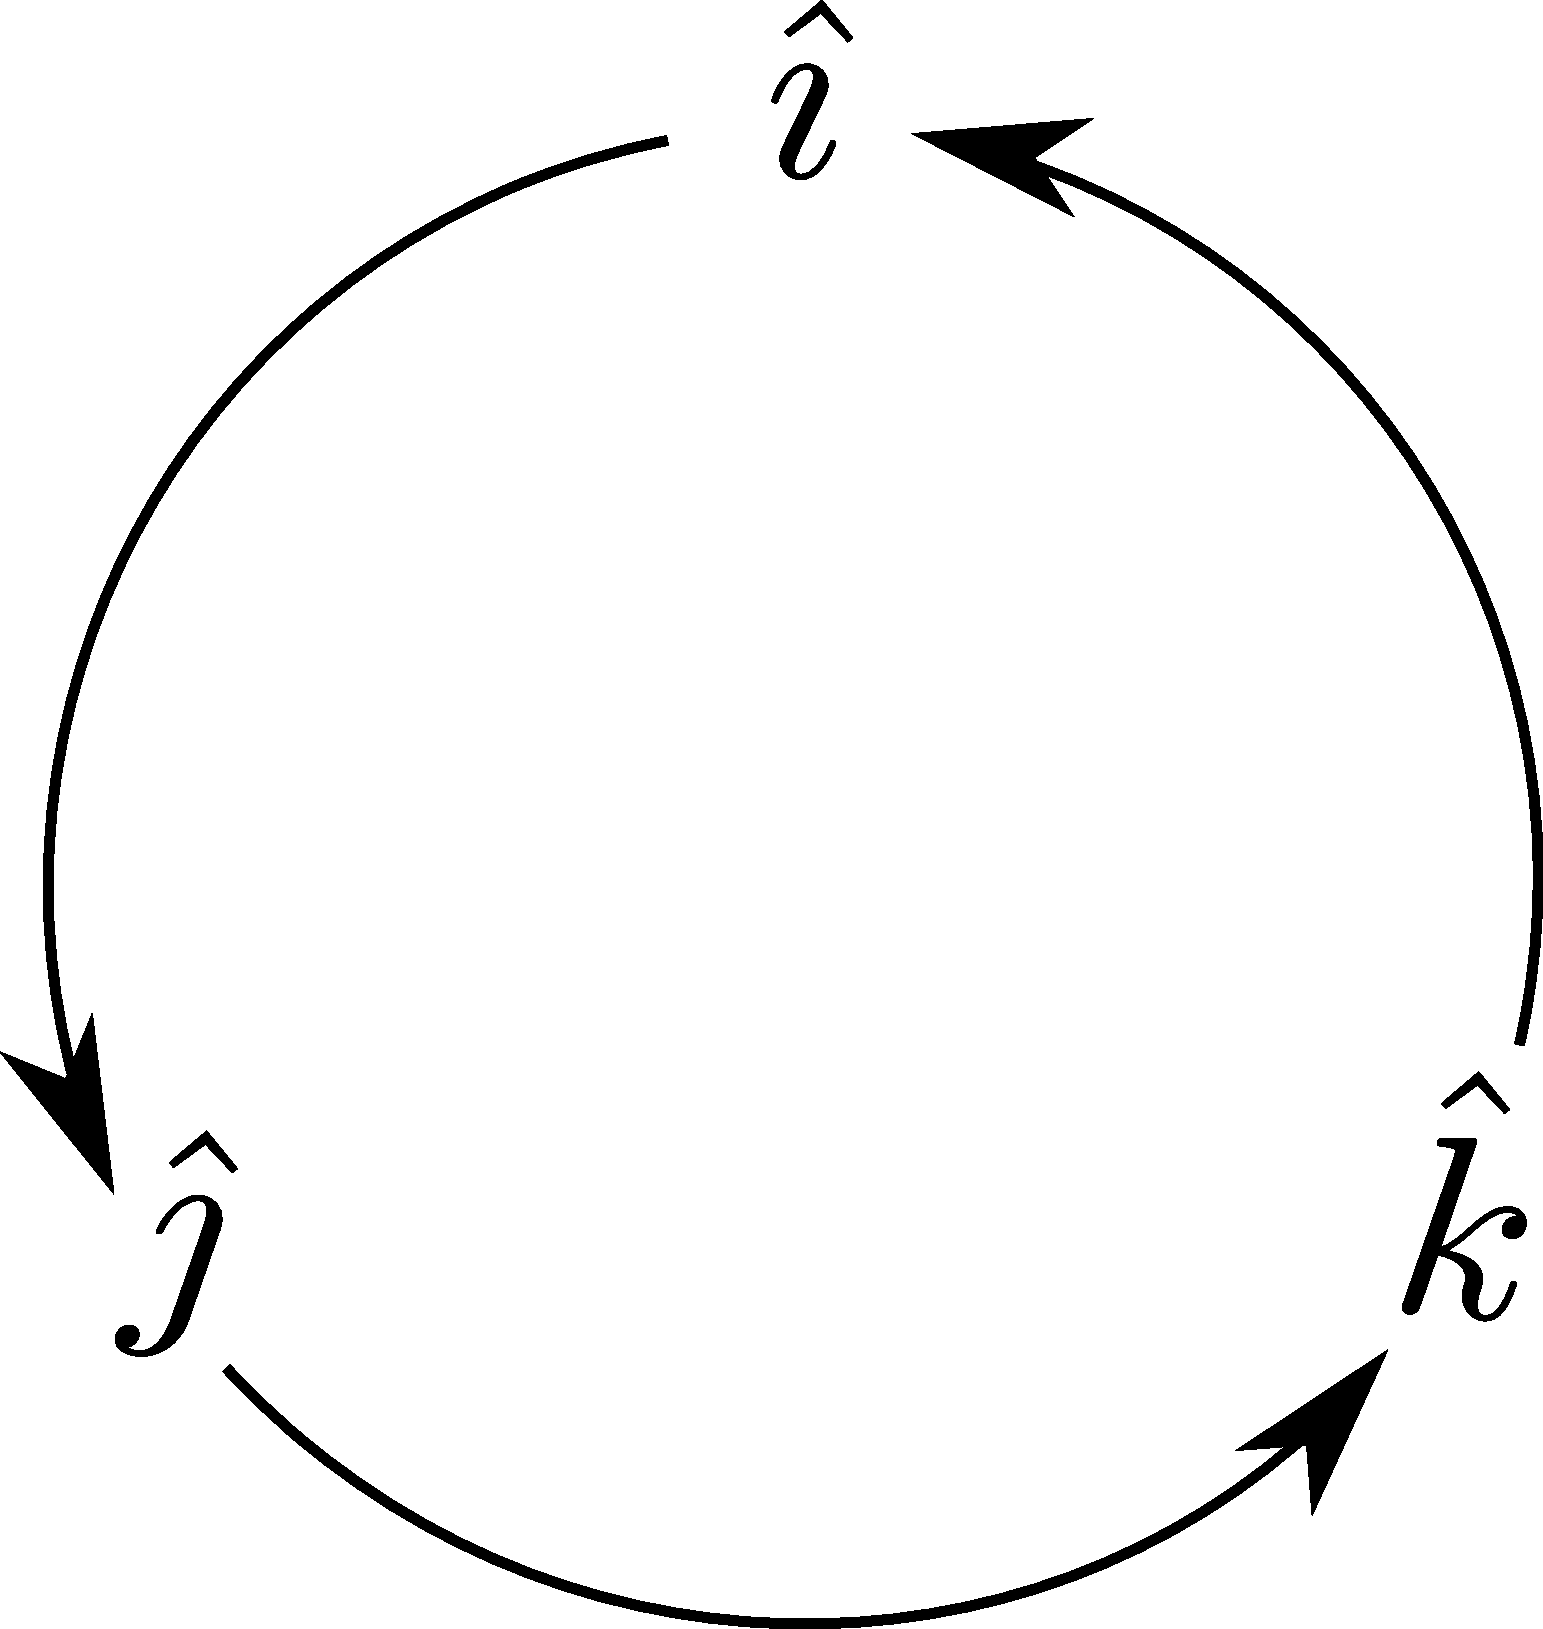
\includegraphics[width=1.5in]{ijk.pdf}
\end{center}

\end{frame}
\begin{frame}\frametitle{Properties of the cross product}
 \begin{theorem}
  If $\vec{u}=\begin{bmatrix}u_1&u_2&u_3\end{bmatrix}^T, \vec{v}=\begin{bmatrix}v_1&v_2&v_3\end{bmatrix}^T,$ and $\vec{w}=\begin{bmatrix}w_1&w_2&w_3\end{bmatrix}^T$, then $\vec{u}\dotp(\vec{v}\times\vec{w}) = \det\begin{bmatrix}u_1&u_2&u_3\\v_1&v_2&v_3\\w_1&w_2&w_3\end{bmatrix}$.
 \end{theorem}
The expression $\vec{u}\dotp(\vec{v}\times \vec{w})$ is often called the \alert{scalar triple product}.
From the above theorem, we can deduce the following:
\begin{itemize}
 \item $\vec{u}\times \vec{v}$ is a vector orthogonal to both $\vec{u}$ and $\vec{v}$.
 \item $\vec{u}\times \vec{0} = \vec{0}\times \vec{u} = \vec{0}$.
 \item If $\vec{u}$ and $\vec{v}$ are parallel, then $\vec{u}\times \vec{v}=\vec{0}$.
 \item $\vec{u}\times \vec{v} = -(\vec{v}\times \vec{u})$.
 \item $(c\vec{u})\times \vec{v} = \vec{u}\times (c\vec{v}) = c(\vec{u}\times \vec{v})$ for any $c\in\R$.
 \item $\vec{u}\times (\vec{v}+\vec{w}) = \vec{u}\times \vec{v}+\vec{u}\times\vec{w}$.
\end{itemize}
\end{frame}
\begin{frame}\frametitle{The Lagrange Identity}
The following result, called the \alert{Lagrange identity}, relates the cross product to the dot product:
\begin{theorem}
 For any two vectors $\vec{u}$ and $\vec{v}$ in $\R^3$, we have
\[
 \len{\vec{u}\times\vec{v}}^2 = \len{\vec{u}}^2\len{\vec{v}}^2-(\vec{u}\dotp\vec{v})^2.
\]
\end{theorem}
Consequence: $\len{\vec{u}\times \vec{v}} = \len{\vec{u}}\len{\vec{v}}\sin\theta$, which is the area of the parallelogram spanned by $\vec{u}$ and $\vec{v}$.
\end{frame}
\begin{frame}\frametitle{Example}
 Find the area of the triangle with vertices $P=(2,1,0)$, $Q=(3,-1,1)$, and $R=(1,0,1)$.
\end{frame}

\begin{frame}\frametitle{Volumes}
 We mentioned in our discussion of determinants that a three-by-three determinant is related to volume. We can see this using the scalar triple product: the vectors $\vec{u},\vec{v},\vec{w}$ span a parallelepided, like so:
\begin{center}
 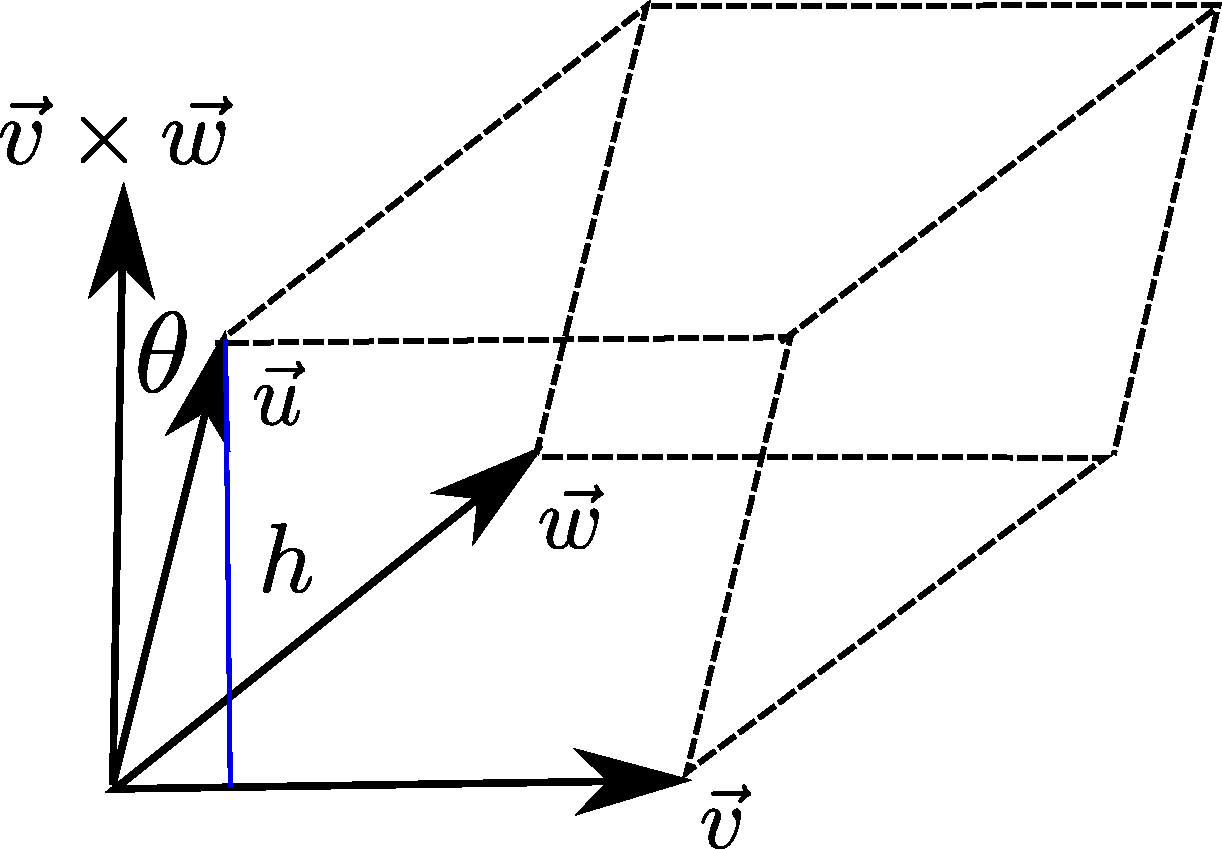
\includegraphics[width=2in]{parallelepiped2.pdf}
\end{center}
The volume is given by $V = Ah$, where $A$ is the area of the base, and $h$ is the height.
\end{frame}
\begin{frame}\frametitle{Example}
 Show that the shortest distance from a point $P$ to the line $L$ through the point $P_0$ with direction vector $\vec{d}$ is
\[
 \frac{\len{\overrightarrow{P_0P}\times\vec{d}}}{\len{\vec{d}}}.
\]

\end{frame}
\begin{frame}\frametitle{Example}
 Find the equation of the plane that contains the lines
\begin{align*}
 L_1: \begin{bmatrix}x\\y\\z\end{bmatrix} &= \begin{bmatrix}1\\-2\\0\end{bmatrix}+s\begin{bmatrix}-2\\3\\1\end{bmatrix}\\
L_2: \begin{bmatrix}x\\y\\z\end{bmatrix} & = \begin{bmatrix}1\\-2\\0\end{bmatrix}+t\begin{bmatrix}3\\-4\\2\end{bmatrix}
\end{align*}

\end{frame}
\begin{frame}\frametitle{Example}
 Find the equation of the plane containing the points $P=(0,1,2)$, $Q=(-2,3,5)$, and $R=(1,1,-3)$.
\end{frame}

\begin{frame}\frametitle{Example}
 Find the distance between the following skew lines, and find the points on each line that are closest together:
\begin{align*}
 \begin{bmatrix}x&y&z\end{bmatrix}^T & = \begin{bmatrix}3&0&1\end{bmatrix}^T+s\begin{bmatrix}2&1&-3\end{bmatrix}^T\\
 \begin{bmatrix}x&y&z\end{bmatrix}^T & = \begin{bmatrix}1&1&-1\end{bmatrix}^T+t\begin{bmatrix}1&0&1\end{bmatrix}^T
\end{align*}

\end{frame}
\section{Orthonormal bases}
\subsection{Subspaces}
\begin{frame}\frametitle{Subspaces}
 Recall: a \alert{subspace} $V\subseteq \R^n$ is a set of vectors in $\R^n$ that contains $\vec{0}$, such that if $\vec{x},\vec{y}\in V$, then $a\vec{x}+b\vec{y}\in V$ for any scalars $a$ and $b$.

\begin{example}
 The set $V=\{(x,y,2x-3y)\,|\, x,y\in\R\}$ is a subspace of $\R^3$.
\end{example}

\vspace{0.5in}

\begin{example}
 Let $\vec{x} = \begin{bmatrix}2&-3&4\end{bmatrix}$ and $\vec{y} = \begin{bmatrix}-1&0&3\end{bmatrix}$ be two vectors in $\R^3$. Then
\[
 \spn\{\vec{x},\vec{y}\} = \{a\vec{x}+b\vec{y}\,|\,a,b\in\R\}
\]
is a subspace of $\R^3$.
\end{example}

\end{frame}
\begin{frame}\frametitle{Spans are subspaces}
 In general, let $\vec{v}_1,\vec{v}_2,\ldots, \vec{v}_k$ be vectors in $\R^n$. Then
\[
 V = \spn\{\vec{v}_1,\vec{v}_2,\ldots, \vec{v}_k\}
\]
is a subspace of $\R^n$.
\end{frame}
\begin{frame}\frametitle{Basis for a subspace}
 One of the most important concepts in linear algebra is that of a \alert{basis}.
\begin{definition}
 Let $V$ be a subspace of $\R^n$. We say that a set of vectors 
\[
B=\{\vec{v}_1,\vec{v}_2,\ldots, \vec{v}_k \}
\]
is a \alert{basis} for $V$ if $\spn B = V$, {\bf and} the vectors in $B$ are linearly independent.
\end{definition}

\end{frame}
\begin{frame}\frametitle{Example}
 Find a basis for the subspace of $\R^3$ defined by the equation $2x-y+3x=0$.

\end{frame}
\begin{frame}\frametitle{Example}
 Find a basis for the subspace
\[
 V = \{(2x-y,x+2y,x,-x+4z)\,|\, x,y\in\R\}\subseteq \R^4
\]

\end{frame}
\subsection{Orthonormal bases}
\begin{frame}\frametitle{Orthogonal sets of vectors}
 Recall that two vectors $\vec{u}$ and $\vec{v}$ are \alert{orthogonal} if $\vec{u}\dotp\vec{v}=0$.
\begin{definition}
 We say that a set $S=\{\vec{v}_1,\vec{v}_2,\ldots, \vec{v}_k\}$ is an \alert{orthogonal set of vectors} if:
\begin{itemize}
 \item $\vec{v}_i\neq \vec{0}$, for all $i=1,2,\ldots, k$,
 \item $\vec{v}_i\dotp \vec{v}_j = 0$ for all $i\neq j$.
\end{itemize}

\end{definition}
\end{frame}

\begin{frame}\frametitle{Example}
Show that the set $\displaystyle \left\{\begin{bmatrix}1\\-2\\0\end{bmatrix},\begin{bmatrix}2\\1\\0\end{bmatrix},\begin{bmatrix}0\\0\\4\end{bmatrix}\right\}$ is an orthogonal set of vectors.
\end{frame}
\begin{frame}\frametitle{Orthogonal sets are linearly independent}
 One reason that orthogonal sets of vectors are useful is that they're automatically linearly independent:
\begin{theorem}
 Let $S=\{\vec{v}_1,\vec{v}_2,\ldots, \vec{v}_k\}$ be an orthogonal set of vectors. Then the vectors in $S$ are linearly independent.
\end{theorem}
\alert{Consequence:} If the vectors in $S$ span a subspace $V$, $S$ is automatically a basis.
\end{frame}
\begin{frame}\frametitle{Fourier and Pythagorus}
 There are two important results involving orthogonal sets of vectors:
\begin{theorem}[Pythogorean Theorem]
 For any set $S=\{\vec{v}_1,\vec{v}_2,\ldots, \vec{v}_k\}$ of orthogonal vectors, we have
\[
 \len{\vec{v}_1+\vec{v}_2+\cdots + \vec{v}_k}^2 = \len{\vec{v}_1}^2+\len{\vec{v}_2}^2+\cdots + \len{\vec{v}_k}^2.
\]
\end{theorem}
\begin{theorem}[Fourier Expansion Theorem]
 Let $S=\{\vec{v}_1,\vec{v}_2,\ldots, \vec{v}_k\}$ be an orthogonal set of vectors. For any $\vec{v}\in \spn S$, we have
\[
 \vec{v} = \left(\frac{\vec{v}_1\dotp\vec{v}}{\len{\vec{v}_1}^2}\right)\vec{v}_1+\left(\frac{\vec{v}_2\dotp\vec{v}}{\len{\vec{v}_2}^2}\right)\vec{v}_2+\cdots +\left(\frac{\vec{v}_k\dotp\vec{v}}{\len{\vec{v}_k}^2}\right)\vec{v}_k
\]

\end{theorem}

\end{frame}

\begin{frame}\frametitle{Orthonormal sets of vectors}
 Recall that a vector $\vec{v}$ is a \alert{unit vector} if $\len{\vec{v}}=1$. For any vector $\vec{u}\neq\vec{0}$, we know that
\[
 \hat{u}=\frac{1}{\len{\vec{u}}}\vec{u}
\]
is a unit vector. (We often say that $\hat{u}$ is \alert{normalized}.) 
\begin{definition}
 We say that a set of vectors $S=\{\vec{v}_1,\vec{v}_2,\ldots, \vec{v}_k\}$ is an \alert{orthonormal set of vectors} if
\[
 \vec{v}_i\dotp \vec{v}_j = \begin{cases} 1, & \text{ if } i=j\\0, & \text{ if } i\neq j\end{cases}.
\]

\end{definition}

\end{frame}
\begin{frame}\frametitle{Orthonormal bases}
\begin{definition}
 Let $V\subseteq \R^n$ be a subspace. We say that $B=\{\vec{v}_1,\vec{v}_2,\ldots, \vec{v}_k\}$ is an \alert{orthonormal basis} (ONB) for $V$ if $\spn B=V$ and $B$ is an orthonormal set of vectors.
\end{definition}
\alert{Note:} Suppose $B$ as above is an orthonormal basis for a subspace $V$. If $v\in V$, then
\[
 v = x_1\vec{v}_1+x_2\vec{v}_2+\cdots + x_k\vec{v}_k
\]
for scalars $x_1,x_2,\ldots, x_k$. In general, finding the values of these scalars requires solving a system of $n$ equations in $k$ variables. For an ONB, it's easy:
 
\end{frame}
\begin{frame}\frametitle{Orthogonal matrices}
 \begin{definition}
  An $n\times n$ matrix $A$ is said to be \alert{orthogonal} if $A^T=A^{-1}$. That is, $A$ satisfies $AA^T=A^TA = I_n$.
 \end{definition}
\begin{theorem}
 An $n\times n$ matrix $A$ is orthogonal if and only if the columns of $A$ form an orthonormal basis of $\R^n$
\end{theorem}
\begin{proof}
 Let $A=[\vec{v}_1|\vec{v}_2|\cdots |\vec{v}_n]$. The $(i,j)$-entry of $A^TA$ is then $\vec{v}_i\dotp\vec{v}_j$.
\end{proof}

\end{frame}
\begin{frame}\frametitle{Example}
 Show that the matrix $A = \begin{bmatrix}\frac{1}{\sqrt{2}}&\frac{1}{\sqrt{6}}&-\frac{1}{\sqrt{3}}\\\frac{1}{\sqrt{2}}&-\frac{1}{\sqrt{6}}&\frac{1}{\sqrt{3}}\\0&\frac{2}{\sqrt{6}}&\frac{1}{\sqrt{3}}\end{bmatrix}$ is orthogonal.
\end{frame}

\begin{frame}\frametitle{Example}
 Let $V\subseteq \R^3$ be the subspace spanned by the vectors $\vec{v}_1 = \begin{bmatrix}3&0&-4\end{bmatrix}^T$ and $\vec{v}_2 = \begin{bmatrix}1&-1&2\end{bmatrix}^T$. Determine if the vector $\vec{v}=\begin{bmatrix}3&-4&2\end{bmatrix}^T$ belongs to $V$.

\bigskip

 \alert{Solution 1}: Solve the system:

\bigskip

\bigskip

 \alert{Solution 2}: Find the normal vector (note $V$ is a plane).

\bigskip

\bigskip

 \alert{Solution 3}: Find an orthogonal basis.
\end{frame}
\subsection{The Gram-Schmidt Procedure}
\begin{frame}\frametitle{Gram-Schmidt}
 The \alert{Gram-Schmidt Procedure} is an algorithm that converts a given basis into an orthonormal basis. The procedure is as follows:

Let $B=\{\vec{v}_1,\ldots, \vec{v}_k\}$ be any basis for a subspace $V\subseteq \R^n$. We define new vectors $\vec{u}_1,\ldots, \vec{u}_k$ as follows:
\begin{align*}
 \vec{u}_1 &= \vec{v}_1.\\
 \vec{u}_2 &= \vec{v}_2 - \operatorname{proj}_{\vec{u}_1}{\vec{v}_2}\\
 \vec{u}_3 &= \vec{v}_3 - \operatorname{proj}_{\vec{u}_1}{\vec{v}_3} - \operatorname{proj}_{\vec{u}_2}{\vec{v}_3}\\
 \vdots & \quad \quad \vdots\\
 \vec{u}_k &= \vec{v}_k - \operatorname{proj}_{\vec{u}_1}{\vec{v}_k} - \operatorname{proj}_{\vec{u}_2}{\vec{v}_k} - \cdots - \operatorname{proj}_{\vec{u}_{k-1}}{\vec{v}_k}
\end{align*}
Then we set $\hat{u}_j = \dfrac{1}{\len{\vec{u}_j}}\vec{u}_j$ for $j=1,\ldots, n$, and the result is an orthonormal set with the same span as $B$.
\end{frame}
\begin{frame}\frametitle{Example}
Suppose a subspace $V\subseteq \R^4$ has the basis  $B=\left\{\begin{bmatrix}1\\0\\1\\0\end{bmatrix},\begin{bmatrix}1\\0\\0\\1\end{bmatrix}, \begin{bmatrix}0\\1\\1\\0\end{bmatrix}\right\}$. Use the Gram-Schmidt procedure to obtain an orthonormal basis.
\end{frame}
\subsection{Orthogonal projection}
\begin{frame}\frametitle{Orthogonal projection}
 Recall: let $V\subseteq \R^n$ be a subspace with orthogonal basis $B= \{\vec{v}_1,\ldots, \vec{v}_k\}$. If $v\in V$, then we have the Fourier expansion
\[
 \vec{v} = \left(\frac{\vec{v}_1\dotp\vec{v}}{\len{\vec{v}_1}^2}\right)\vec{v}_1+\left(\frac{\vec{v}_2\dotp\vec{v}}{\len{\vec{v}_2}^2}\right)\vec{v}_2+\cdots +\left(\frac{\vec{v}_k\dotp\vec{v}}{\len{\vec{v}_k}^2}\right)\vec{v}_k.
\]
What if $\vec{v}\notin V$? If that's the case, then the right-hand side above can't equal $\vec{v}$ (since  it belongs to $V$). What we get instead is the \alert{orthogonal projection} $\operatorname{proj}_V\vec{v}$ of $\vec{v}$ onto $V$.
\begin{theorem}
 Let $\vec{w}=\operatorname{proj}_V\vec{u}$ be the orthogonal projection of $\vec{u}$ onto a subspace $V$ with respect to an orthogonal basis. Then $\vec{w}$ is the closest point in $V$ to $\vec{u}$. (That is, $\len{\vec{w}-\vec{u}}$ is as small as possible.)
\end{theorem}

\end{frame}
\begin{frame}\frametitle{Example}
 Let $V\subseteq \R^3$ be the plane spanned by the vectors $\vec{v} = \begin{bmatrix}0&-3&4\end{bmatrix}^T$ and $\vec{w} = \begin{bmatrix}2&-1&2\end{bmatrix}$. Find the point in $V$ that is closest to the point $P=(2,0,4)$.
\end{frame}
\begin{frame}\frametitle{Orthogonal complement}
 Let $V\subseteq \R^n$ be a subspace. We define the \alert{orthogonal complement} $V^\bot$ of $V$ to be the set
\[
 V^\bot = \{\vec{w}\in \R^n \,|\, \vec{w}\dotp\vec{v} = 0 \text{ for all }\vec{v}\in V\}.
\]
 \begin{theorem}
  If $V$ is a subspace, then $V^\bot$ is also a subspace. Moreover, every $\vec{x}\in\R^n$ can be written \alert{uniquely} in the form $\vec{x} = \vec{v}+\vec{w}$, where $\vec{v}\in V$ and $\vec{w}\in V^\bot$.
 \end{theorem}
 
\end{frame}
\begin{frame}\frametitle{Finding $V^\bot$}
 Given a subspace $V$, how do we find $V^\bot$? First, suppose $B=\{\vec{v}_1,\ldots, \vec{v}_k\}$ is a basis for $V$. If $\vec{w}\in V^\bot$, then we must have
\[
 \vec{w}\dotp \vec{v}_1 = 0, \vec{w}\dotp \vec{v}_2 = 0,\ldots, \vec{w}\dotp\vec{v}_k=0.
\]
But this is just a system of $k$ \alert{homogeneous} linear equations in $n$ variables, with $k\leq n$.
\end{frame}
\begin{frame}\frametitle{Examples}
 Find the orthogonal complement of:

(a) $V = \{(t,-2t,3t)\,|\,t\in\R\}\subseteq \R^3$.

(b) $V = \{(x,y,z)\,|\, 2x-y+3z=0\}\subseteq \R^3$.

\end{frame}






\end{document}